% Created 2020-08-07 Fri 14:24
% Intended LaTeX compiler: pdflatex
\documentclass[presentation]{beamer}
\usepackage[utf8]{inputenc}
\usepackage[T1]{fontenc}
\usepackage{graphicx}
\usepackage{grffile}
\usepackage{longtable}
\usepackage{wrapfig}
\usepackage{rotating}
\usepackage[normalem]{ulem}
\usepackage{amsmath}
\usepackage{textcomp}
\usepackage{amssymb}
\usepackage{capt-of}
\usepackage{hyperref}
\usetheme{UoB}
\author{Mark Blyth}
\date{\textit{[2020-08-10 Mon]}}
\title{Broken codes}
\hypersetup{
 pdfauthor={Mark Blyth},
 pdftitle={Broken codes},
 pdfkeywords={},
 pdfsubject={},
 pdfcreator={Emacs 26.3 (Org mode 9.1.9)}, 
 pdflang={English}}
\begin{document}

\maketitle

\section{Background}
\label{sec:org1da686e}
\begin{frame}[label={sec:org376d3dc}]{Week's work}
\begin{itemize}
\item Redraft continuation review
\item Run in-silico CBC with Fourier, splines
\begin{itemize}
\item Doesn't work
\item Simplest case (Fourier, Duffing) doesn't work either
\end{itemize}
\end{itemize}
\end{frame}
\section{Pictures of code not working}
\label{sec:org6df7608}
\begin{frame}[label={sec:org59dcc17}]{No controller, no orthogonality constraint}
Code fits a discretisation to the uncontrolled system output; useful to test Newton convergence

\begin{center}
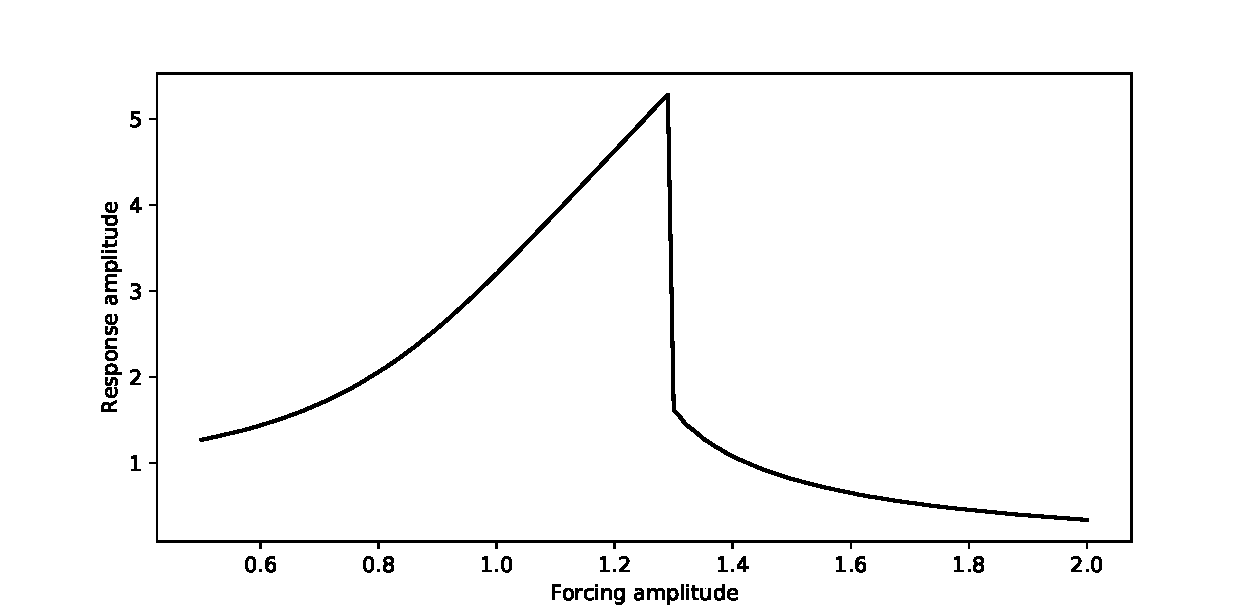
\includegraphics[width=.9\linewidth]{./nonorthogonal-controlfree.pdf}
\end{center}
\end{frame}

\begin{frame}[label={sec:orgda4cf77}]{No controller, orthogonality constraint}
Code fits a discretisation to the uncontrolled system output, with psuedo-arclength regularisation; fails in the expected way

\begin{center}
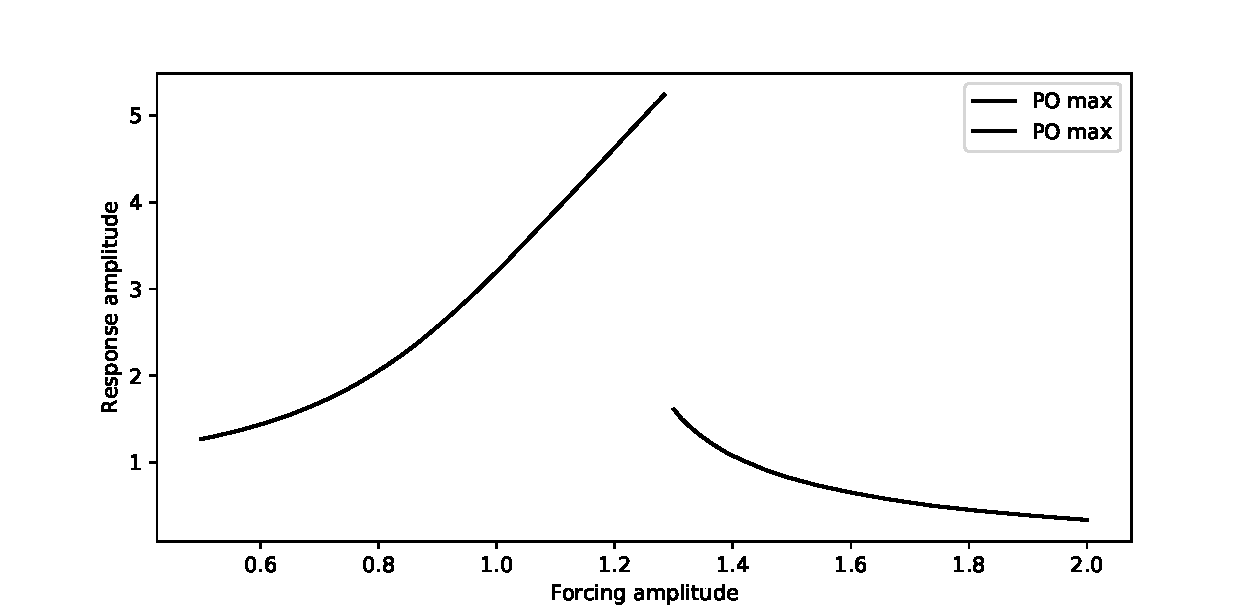
\includegraphics[width=.9\linewidth]{./controlfree_continuation.pdf}
\end{center}
\end{frame}

\begin{frame}[label={sec:orgf24aef9}]{Full control-based continuation}
\begin{center}
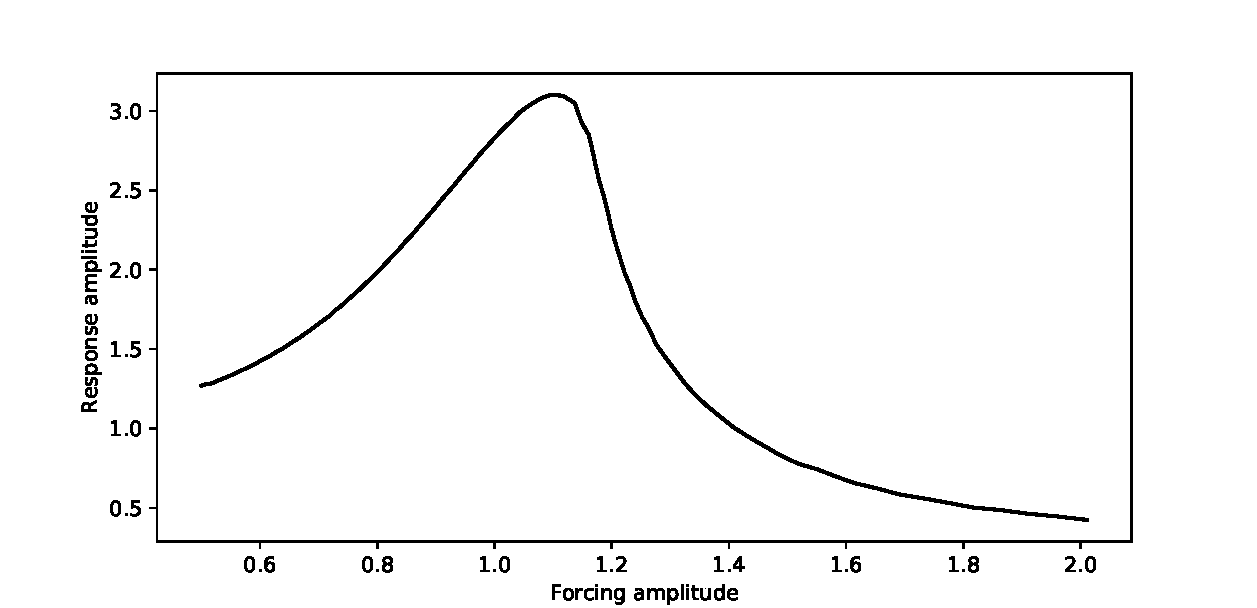
\includegraphics[width=.9\linewidth]{./failed_duffing.pdf}
\end{center}
\end{frame}

\begin{frame}[label={sec:org13035e4}]{System inputs and outputs match properly}
\begin{center}
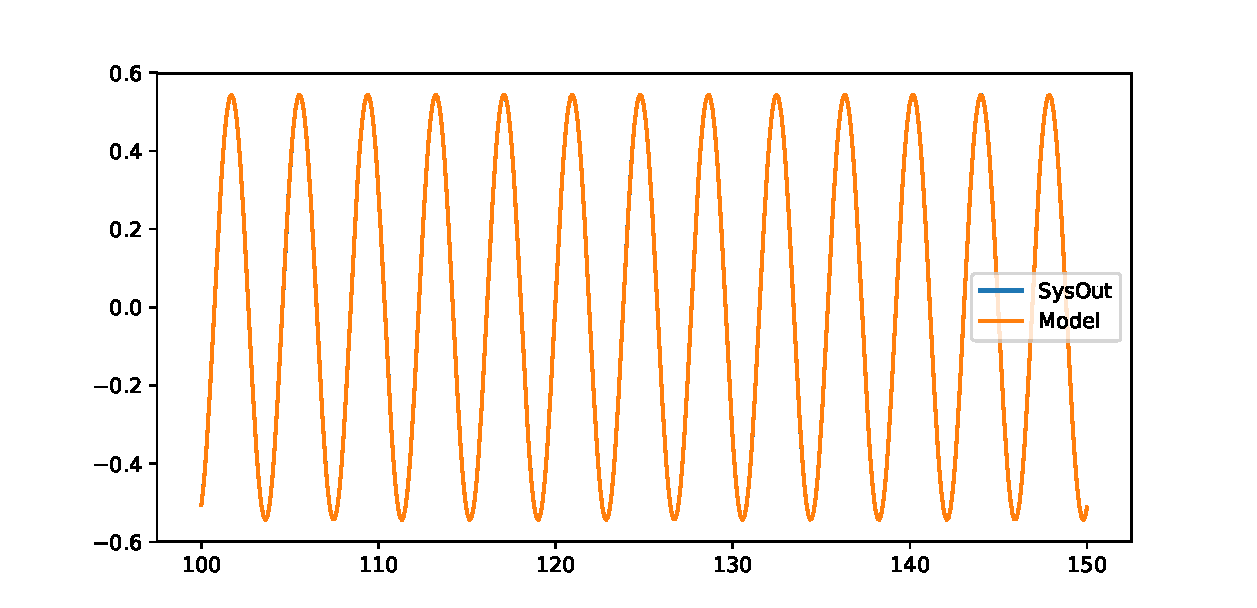
\includegraphics[width=.9\linewidth]{./trial.pdf}
\end{center}
\end{frame}

\begin{frame}[label={sec:org6f81666}]{Fitzhugh Nagumo control-based continuation}
\begin{center}
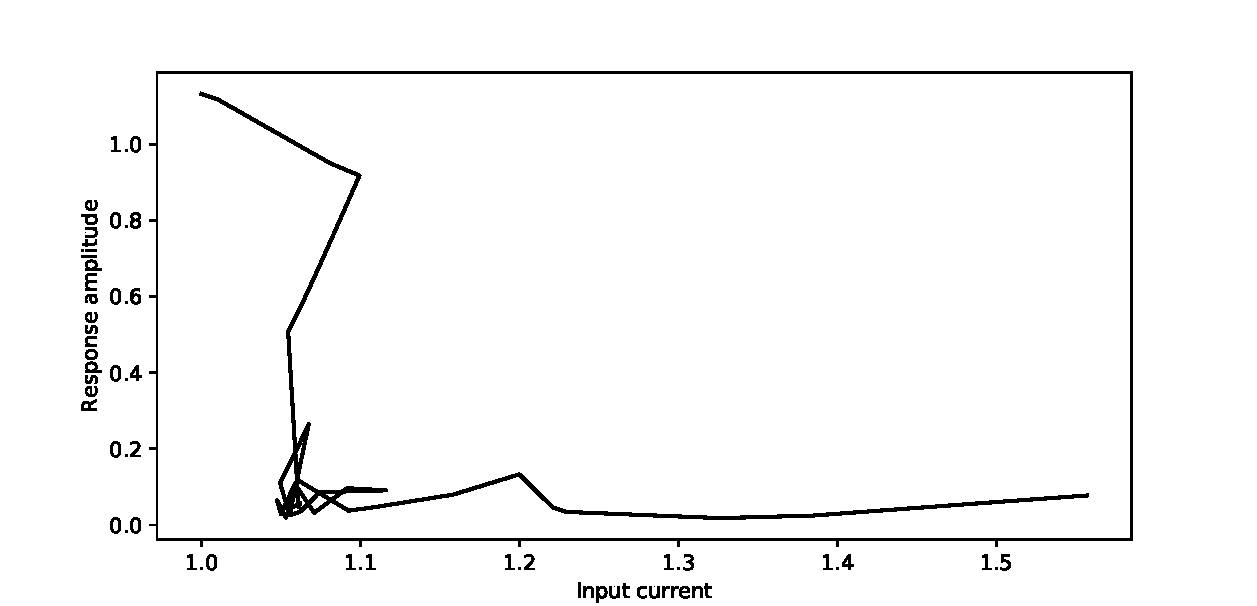
\includegraphics[width=.9\linewidth]{./FH_CBC.pdf}
\end{center}
\end{frame}

\begin{frame}[label={sec:org0d15fef}]{Tests}
\begin{itemize}
\item Reduced it to simplest possible code / maths
\item Checked continuation system against the literature
\item Checked controlled systems work properly
\item Checked discretisations match signals properly
\item Tried different RHS's (Duffing, Fitzhugh Nagumo, `weak' Fitzhugh Nagumo)
\item Played with hyperparameters (control gains, step size)
\end{itemize}
\end{frame}

\begin{frame}[label={sec:org50e72e9}]{Next steps}
\begin{itemize}
\item House moving
\item Start writing conference paper
\begin{itemize}
\item Figure out best coding approach based on that
\end{itemize}
\end{itemize}
\end{frame}
\end{document}
